%!TEX root = ../rapport.tex
%!TEX encoding = UTF-8 Unicode

% Chapitres "Introduction"

% modifié par Francis Valois, Université Laval
% 31/01/2011 - version 1.0 - Création du document


\label{s:experimentation}
\chapter{Laboratoire 2}
\section{Projet 1}
Nous avons choisi une charge de valeur 100$\Omega$ puisque pour cette valeur, on obtient un coefficient de réflexion théorique faible. Pour affirmer cela, on utilise l'expression suivante:
\begin{equation}
\Gamma_g (s) = \frac{Z_g(s) - Z_0(s)}{Z_g(s) + Z_0(s)}
 \end{equation} 

\paragraph{}Dans le circuit étudié, on cherche à avoir $Z_0$ (l'impédance mise en parallèle avec la source) $\approx Z_G$ (l'impédance de la ligne)

\paragraph{}Afin d'observer de manière pratique le comportement des réflexions du circuit, nous avons essayé chacune des résistance disponible dans les choix en plus de celle de 100$\Omega$. Nous présenterons les courbes obtenus à l'oscilloscope à l'annexe \ref{s:annexes}. Comme seule la courbe pour la résistance de 100$\Omega$ est requise selon l'énoncé de laboratoire, elle est présentée ci-dessous:

\begin{figure}[htb]
\begin{center}
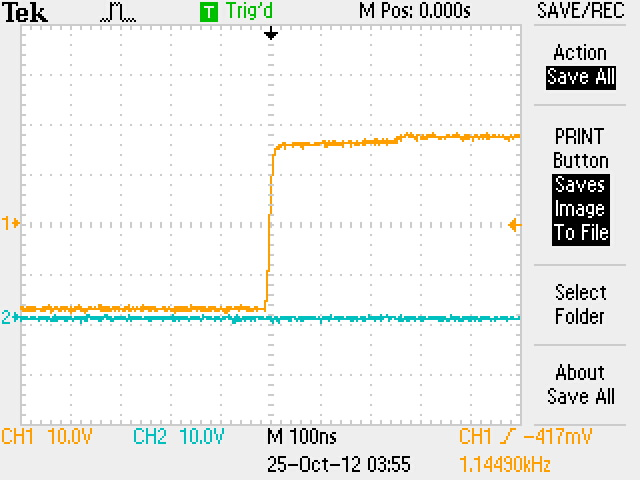
\includegraphics[scale=0.3]{Reflexion_R_100.jpg}
\caption{Courbes obtenus à l'oscilloscope pour le projet 1 en utilisant une résistance de 100 $\Omega$}
\label{Reflexion_R_100}
\end{center}
\end{figure}

On note dans cette figure que la réflexion est bel et bien faible, mais existante, en utilisant une résistance variable (le potentiomètre), on lit au multimètre une résistance très proche de 93$\Omega$. Cette résistance est très proche de l'impédance intrinsèque de ligne du tableau 1 présenté dans le protocle de laboratoire( $z_0 = 93\Omega$). L'ensemble des autres courbes est présenté dans l'annexe \ref{s:annexes}

\paragraph{}On remarque que la valeur fournie par le manufacturier est très précise. La différence entre la valeur du manufacturier et celle mesurée repose sur le bruit du signal qui affecte la précision de la lecture à l'oscilloscope et aussi la précision limitée de l'instrument de mesure de la résistance. 
\newpage
\section{Projet 2}

Dans ce projet, il était demandé de visualiser simultanément les signaux au niveau de la charge et de la source sur la ligne RG-58 de 30m. Cela fut fait pour des charges de respectivement 0 $\Omega$, 27 $\Omega$ et 50$\Omega$. Les courbes obtenues sont présentées aux figures suivantes:

\begin{figure}[htb]
	\centering
\subfigure[Régime transitoire pour $R = 0 \Omega$]{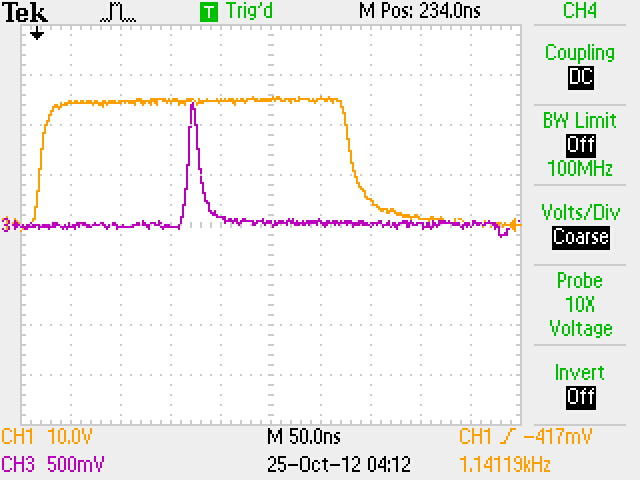
\includegraphics[scale =0.3]{fig/TR0.JPG} \label{fig:transr0}}
		\quad
		\subfigure[Front montant du régime transitoire pour $R = 27 \Omega$]{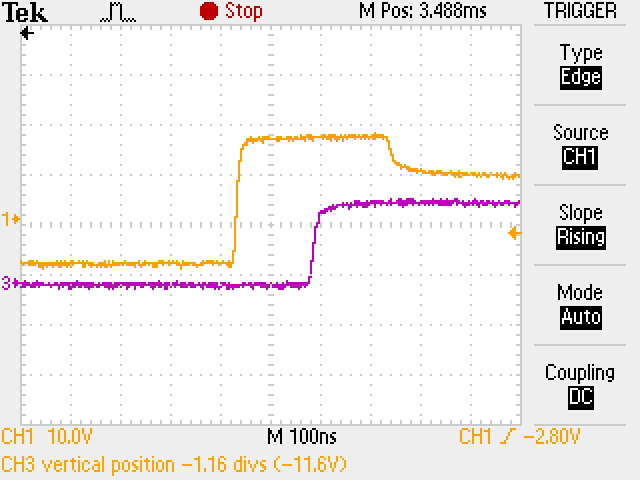
\includegraphics[scale =0.3]{fig/TR272.JPG} \label{fig:transr272}}
		\quad
		\subfigure[Front descendant du régime transitoire pour $R = 27 \Omega$]{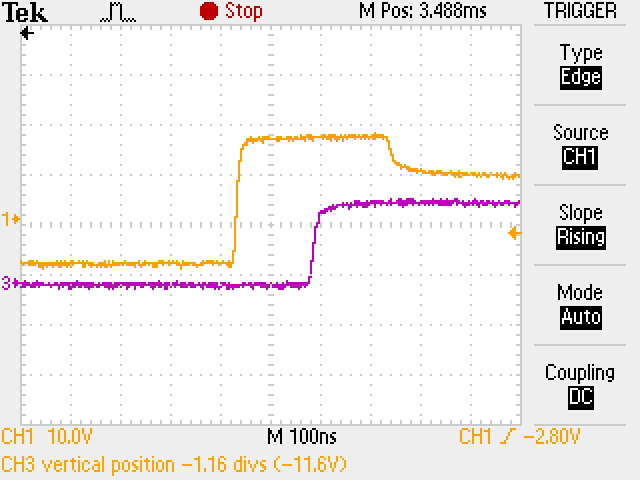
\includegraphics[scale =0.3]{fig/TR272.JPG} \label{fig:transr271}}
		\quad
		\subfigure[Vue d'ensemble du régime transitoire pour $R = 27 \Omega$]{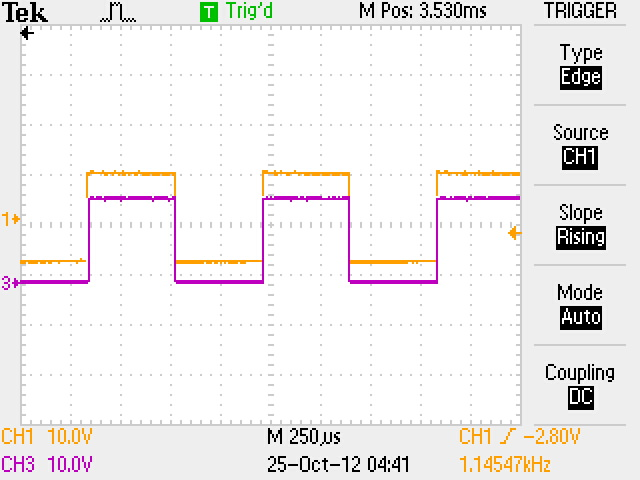
\includegraphics[scale =0.3]{fig/TR273.JPG} \label{fig:transr273}}
\end{figure}

\section{Projet 3: Reproduction des exemples}
\newpage
\section{Projet 4: Résultats obtenus selon la géométrie et les diélectriques}


